\documentclass{beamer}
\usetheme{Warsaw}

\usepackage{graphicx} % Allows including images
\usepackage{booktabs} % Allows the use of \toprule, \midrule and \bottomrule in tables
\usepackage{listings}
\usepackage[utf8]{inputenc}
\usepackage[overlay,absolute]{textpos}
\usepackage{tikz}
\usetikzlibrary{arrows}

\AtBeginSection[]
{
\begin{frame}<beamer>
\frametitle{Plan}
\tableofcontents[
  currentsection,
  hideothersubsections
]
\end{frame}
}

\lstset{language=C++,
                basicstyle=\ttfamily,
                keywordstyle=\color{green}\ttfamily,
                stringstyle=\color{red}\ttfamily,
                commentstyle=\color{cyan}\ttfamily,
                morecomment=[l][\color{magenta}]{\#},
                escapechar=@
}

\setbeamercolor{normal text}{fg=white,bg=black!90}
\setbeamercolor{structure}{fg=white}

\setbeamercolor{alerted text}{fg=red!85!black}

\setbeamercolor{item projected}{use=item,fg=black,bg=item.fg!35}

\setbeamercolor*{palette primary}{use=structure,fg=structure.fg}
\setbeamercolor*{palette secondary}{use=structure,fg=structure.fg!95!black}
\setbeamercolor*{palette tertiary}{use=structure,fg=structure.fg!90!black}
\setbeamercolor*{palette quaternary}{use=structure,fg=structure.fg!95!black,bg=black!80}

\setbeamercolor*{framesubtitle}{fg=white}

\setbeamercolor*{block title}{parent=structure,bg=black!60}
\setbeamercolor*{block body}{fg=black,bg=black!10}
\setbeamercolor*{block title alerted}{parent=alerted text,bg=black!15}
\setbeamercolor*{block title example}{parent=example text,bg=black!15}

\author[Félix-Antoine Ouellet]{Félix-Antoine Ouellet}

\title[Functional\hspace{2em}\insertframenumber/\inserttotalframenumber]{C++ Fonctionnel}

\date{24 octobre 2015}

\begin{document}

\begin{frame}
\titlepage % Print the title page as the first slide
\end{frame}

\begin{frame}
\frametitle{Disclaimer}
\begin{center}

\includegraphics[scale=0.49]{dude.jpg}
\end{center}
\end{frame}

\begin{frame}
\frametitle{}
\begin{center}
\Huge{\textbf{ENTREVUE}}
\end{center}
\end{frame}

\begin{frame}
\frametitle{Question 0}
\begin{center}
\Huge{Implémenter Fibonacci}
\end{center}
\end{frame}

\begin{frame}
\frametitle{Question 1}
\begin{center}
\Huge{Implémenter Fibonacci avec une lambda}
\end{center}
\end{frame}

\begin{frame}
\frametitle{Question 2}
\begin{center}
\Huge{Accélérer Fibonacci}
\end{center}
\end{frame}

\begin{frame}
\frametitle{Question 3}
\begin{center}
\Huge{Accélérer Fibonacci (encore!)}
\end{center}
\end{frame}

\begin{frame}
\frametitle{Question 4}
\begin{center}
\Huge{Accélérer Fibonacci (ENCORE!)}
\end{center}
\end{frame}

\begin{frame}
\frametitle{Template Metaprogramming}
\begin{center}
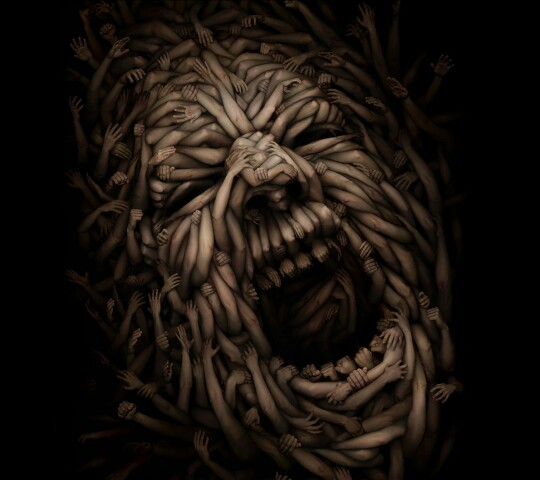
\includegraphics[scale=0.4]{TMP.jpg}
\end{center}
\end{frame}

\begin{frame}
\frametitle{Question 5}
\begin{center}
\Huge{Version lisible pour le commun des mortels?}
\end{center}
\end{frame}

\begin{frame}
\frametitle{Question 6}
\begin{center}
\Huge{Composition}
\end{center}
\end{frame}

\begin{frame}
\frametitle{Question 7}
\begin{center}
\Huge{Fibonacci infini}
\end{center}
\end{frame}

\begin{frame}
\frametitle{Question 8}
\begin{center}
\Huge{Composition infinie}
\end{center}
\end{frame}

\begin{frame}
\frametitle{Merci}
\begin{center}
\Huge{\textbf{Applaudissez!}}
\end{center}
\end{frame}

\end{document}